\usepackage{etex} %эта магическая херь избавляет от переполнения регистров TeX а!!!

\mode<article>{\usepackage{fullpage}}
\mode<presentation>{
    \usetheme{Madrid}
    \useoutertheme{shadow}
} 

\usepackage[utf8]{inputenc}
\usepackage[russian]{babel}
\usepackage{indentfirst}
\usepackage{graphicx}

\usepackage{amsmath}
\usepackage{amsfonts}
\usepackage{amsthm}
%\usepackage{algorithm}
%\usepackage{algorithmic}

%\usepackage[all]{xy}

\date{Лекция по дисциплине <<методы и средства защиты компьютерной информации>> (\today)}
\author[М.~М.~Шихов]{Михаил Шихов \\ \texttt{\underline{m.m.shihov@gmail.com}}}

%%для рисования графов пакетом xy-pic
%\entrymodifiers={++[o][F-]}

%%для псевдокода алгоритмов (algorithm,algorithmic)
%\renewcommand{\algorithmicrequire}{\textbf{Вход:}}
%\renewcommand{\algorithmicensure}{\textbf{Выход:}}
%\renewcommand{\algorithmiccomment}[1]{// #1}
%\floatname{algorithm}{Псевдокод}

%\setbeamercolor{alerted text}{fg=-green} %gyan, blue, green, -green

\title[Математические основы криптографии]{Математические основы криптографии}


\begin{document}


\mode<article>{\maketitle\tableofcontents}


\frame<presentation>{\titlepage}
\begin{frame}<presentation>[allowframebreaks]
\frametitle{Содержание}
\tableofcontents
\end{frame}


\section{Группы, кольца, поля}


\subsection{Группа}


\begin{frame}
    \frametitle{Группа}
    \begin{definition}
        Множество $A$ образует \alert{группу}, если на нем определена бинарная операция $\circ:A\times A\to A$ и для всех элементов $a,b,c\in A$ выполняются следующие аксиомы.
        \begin{enumerate}
            \item \label{en:groupClosure}\alert{Замкнутость}. $a \circ b \in A$.
            \item \label{en:groupAssoc}\alert{Ассоциативность}. $(a \circ b) \circ c =  a \circ (b \circ c)$.
            \item \label{en:groupNeytral} \alert{Тождество}. Имеется \alert{нейтральный} элемент $e\in A$ такой, что: $e \circ a = a \circ e = a$.
            \item \label{en:groupNegative} \alert{Инверсия}. Имеется \alert{обратный} элемент $a^{-1}\in A$ для каждого $a$, такой, что: $a^{-1} \circ a = a \circ a^{-1} = e$.
            \item<2-> Если операция еще и \alert{коммутативна}: $a \circ b = b \circ a$, то группа называется \alert{абелевой}.
        \end{enumerate}
    \end{definition}
\end{frame}

\alert{Полугруппа} --- это группа, для которой выполняются аксиомы \ref{en:groupClosure},\ref{en:groupAssoc}. \alert{Моноид} --- это группа, для которой выполняются аксиомы \ref{en:groupClosure},\ref{en:groupAssoc},\ref{en:groupNeytral}.

Примеры групп: 
\begin{itemize}
    \item Множество целых чисел --- группа, относительно сложения, как и множества рациональных, действительных и комплексных чисел. Нейтральный элемент --- ноль.
    \item Ненулевые элементы множеств целых, рациональных, дейтсвительных и комплексных чисел --- группа по умножению. Нейтральный элемент --- единица.
    \item Группа часовой стрелки по сложению.
\end{itemize}


\subsection{Кольцо}


\begin{frame}
    \frametitle{Кольцо}
    
    \begin{definition}
        Множество $R$ образует \alert{кольцо}, если на нем определены \alert{две} операции \alert{сложение} $+$ и \alert{умножение} $\cdot$, обладающие для $a,b,c\in R$ следующими свойствами.
        \begin{enumerate}
            \item Относительно \alert{сложения} $+$ кольцо $R$ образует \alert{абелеву} группу. Нейтральный элемент (ноль) обозначается символом $0$.
            \item Относительно \alert{умножения} $\cdot$ кольцо $R$ удовлетворяет аксиомам \alert{замктутости}, \alert{ассоциативности}.
            \item Аксиома \alert{дистрибутивности}. $a\cdot(b+c) = a\cdot b + a\cdot c$
            \item<2-> Кольцо называтся \alert{коммутативным}, если опереция \alert{умножения} комутативна: $a\cdot b = b\cdot a$.
            \item<3-> Кольцо называется кольцом \alert{с единицей}, если имеется нейтральный элемент по умножению (единица). Нейтральный элемент обозначается символом $1$.
        \end{enumerate}
    \end{definition}
\end{frame}


\subsection{Поле}


\begin{frame}
    \frametitle{Поле}
    
    \begin{definition}
        Множество $F$ образует \alert{поле}, если оно является \alert{коммутативным кольцом} и его ненулевые элементы образуют \alert{группу} относительно операции \alert{умножения}.
    \end{definition}
	
	Элемент, \alert{обратный} элементу $a$ по сложению обозначается $-a$; \alert{обратный} по умножению --- $a^{-1}$.

    Иногда дополнительно вводят операции \alert{вычитания}: \[a-b=a+(-b)\] и \alert{деления}: \[\frac{a}{b}=a\cdot b^{-1}.\]
\end{frame}


В высшей алгебре доказывается, что число элементов $q$ конечного поля (которое называется полем Галуа\footnote{Эварист Галуа француз в написал все свои математические работы в возрасте до 20 лет. Был убит на дуэли}) удовлетворяет соотношению $q = p^m$. Где $p$ --- простое число. А $m$ принадлежит диапазону целых чисел $[1, \infty)$.

Наиболее просто обстоит дело с $m=1$. Тогда элементы поля есть числа $\{0,1,\ldots,p-1\}$. Рассмотрим небольшой пример поля. Выберем простое $p=5, m=1$ и построим конечную группу. Элементы такой группы будут принадлежать множеству $\{0, 1, 2, 3, 4\}$. А операции сложения и умножения будут выполняться по модулю 5 $pmod{5}$. Т.е иногда мы будем говорить, что $7 = 2$ не уточняя, что $7 \equiv 2 \mod{5}$. Т.е. $7$ будет принадлежать классу эквивалентности $2$.


\begin{frame}
    \frametitle{Пример конечного поля}
    
    \begin{columns}
        \column{.45\textwidth}
        \begin{block}{Сложение}
            \begin{table}[ht]
                \mode<article>{\caption{Сложение}}\label{t:fieldAddDgt}
                \centering
                \begin{tabular}[c]{|l||l|l|l|l|l|}
                    \hline
                    +& 0& 1& 2& 3& 4\\ \hline\hline 
                    0& 0& 1& 2& 3& 4\\ \hline 
                    1& 1& 2& 3& 4& 0\\ \hline 
                    2& 2& 3& 4& 0& 1\\ \hline 
                    3& 3& 4& 0& 1& 2\\ \hline 
                    4& 4& 0& 1& 2& 3\\ \hline 
                \end{tabular}
            \end{table}
            \[c\equiv a+b \pmod{5}\]
        \end{block}
        
        \column{.45\textwidth}
        \begin{block}{Умножение}
            \begin{table}[ht]
                \mode<article>{\caption{Умножение}}\label{t:fieldMulDgt}
                \centering
                \begin{tabular}[c]{|l||l|l|l|l|l|}
                    \hline
                    $\cdot$ & 0& 1& 2& 3& 4\\ \hline\hline
                    0       & 0& 0& 0& 0& 0\\ \hline 
                    1       & 0& 1& 2& 3& 4\\ \hline 
                    2       & 0& 2& 4& 1& 3\\ \hline 
                    3       & 0& 3& 1& 4& 2\\ \hline 
                    4       & 0& 4& 3& 2& 1\\ \hline 
                \end{tabular}
            \end{table}
            \[c\equiv a\cdot b \pmod{5}\]
        \end{block}
    \end{columns}
    \mode<article>{Сложение см. \ref{t:fieldAddDgt}, умножение см. \ref{t:fieldMulDgt}}
\end{frame}


Для пущей общности, введем обозначения цифр буквами, чтобы показать, что элементами конечного поля могут быть не обязательно числа.


\begin{frame}
    \frametitle{Пример конечного поля}
    
    В поле Галуа $GF(p)$ имеется по крайней мере один \alert{примитивный} элемент $\alpha$, такой, что любой \alert{ненулевой} элемент \alert{поля} может быть представлен как степень $\alpha^n=\underbrace{\alpha\cdot\alpha\cdot\ldots\cdot\alpha}_n$.
    
    \begin{columns}
        \column{.45\textwidth}
        \begin{block}{Сложение}
            \begin{table}[ht]
                \mode<article>{\caption{Сложение}}\label{t:fieldAdd}
                \centering
                \begin{tabular}[c]{|l||l|l|l|l|l|}
                        \hline
                        +& a& b& c& d& f\\ \hline\hline
                        a& a& b& c& d& f\\ \hline
                        b& b& c& d& f& a\\ \hline
                        c& c& d& f& a& b\\ \hline
                        d& d& f& a& b& c\\ \hline
                        f& f& a& b& c& d\\ \hline
                \end{tabular}
            \end{table}
        \end{block}
        
        \column{.45\textwidth}
        \begin{block}{Умножение}
            \begin{table}[ht]
                \mode<article>{\caption{Умножение}}\label{t:fieldMul}
                \centering
                \begin{tabular}[c]{|l||l|l|l|l|l|}
                    \hline
                    $\cdot$ & a& b& c& d& f\\ \hline\hline
                    a       & a& a& a& a& a\\ \hline
                    b       & a& b& c& d& f\\ \hline
                    c       & a& c& f& b& d\\ \hline
                    d       & a& d& b& f& c\\ \hline
                    f       & a& f& d& c& b\\ \hline
                \end{tabular}
            \end{table}
        \end{block}
    \end{columns}
    \mode<article>{Сложение см. \ref{t:fieldAdd}, умножение см. \ref{t:fieldMul}}
    
    \uncover<2->{В данном примере поля \alert{два} примитивных элемента:} \uncover<3->{$c$ и $d$.}
\end{frame}


\section{Примеры алгебраических систем}


\subsection{Арифметика остатков}

\begin{frame}
    \frametitle{Арифметика остатков}
    \framesubtitle{Введение}
    
    Фиксируется положительное натуральное число $N$, которое и называется \alert{модулем}. Если разность двух целых чисел $a-b$ делится на $N$ нацело, то пишут \[a\equiv b \pmod{N}.\]
    
    Такие числа $a$ и $b$ называются \alert{сравнимыми} по модулю \alert{$N$}. В этом случае числа $a$ и $b$ имеют, очевидно одинаковый остаток от деления на $N$.
    \[18\equiv 4\pmod{7}, -18\equiv 3\pmod{7}\]
    Все возможные остатки от деления на $N$ образуют множество\footnote{Иногда обозначается как $\mathbb{Z}_N$} \[\mathbb{Z}/N\mathbb{Z}=\{0,\ldots,N-1\}.\]
    Элемент $x\in\mathbb{Z}/N\mathbb{Z}$ <<изображает>> целый класс чисел $x+kN,k\in \mathbb{Z}$.
\end{frame}


\begin{frame}
    \frametitle{Арифметика остатков}
    \framesubtitle{Кольцо вычетов по модулю $N$}
    
    На множестве $\mathbb{Z}/N\mathbb{Z}$ вводятся две операции --- \alert{сложение} и \alert{умножение}. Они определяются обычным путем, например,
    \[\underbrace{11+13}_{24}\equiv 8 \pmod{16},\] так как $24=1\cdot 16 + 8$, и 
    \[\underbrace{11\cdot 13}_{143}\equiv 15 \pmod{16},\] так как $143=8\cdot 16 + 15$.
    
    Таким образом, $\mathbb{Z}/N\mathbb{Z}$ является \alert{коммутативным кольцом} и называется в литературе \alert{кольцом вычетов по модулю $N$}.
\end{frame}


\begin{frame}
    \frametitle{Арифметика остатков}
    \framesubtitle{Сложные задачи}
    
    В криптографии активно используются \alert{трудноразрешимые}\footnote{Имеющие вычислительную сложность $O(2^n)$, $O(n!)$ и т.д.} задачи.
    \begin{itemize}
        \item Задача разложения натурального числа $N$ на простые сомножители
            \[N=\prod_{i=1}^{m}p_i^{k_i},\]
            где $p_i$ --- простой сомножитель, $k_i$ --- его степень.
        \item Задача дискретного логарифмирования в кольце вычетов по модулю $N$
            \[y\equiv a^x\pmod{N}.\]
    \end{itemize}
\end{frame}


\begin{frame}
    \frametitle{Арифметика остатков}
    \framesubtitle{Сопутствующие простые задачи}
    
    Сложность порядка $O(\log_2m)$ имеют сопутствующие задачи\footnote{См. подробнее в приложении}. 
    \begin{itemize}
        \item Поиск мультипликативного обратного $x=a^{-1}$
            \[a\cdot x\equiv 1\pmod{m}\]
        выполняется с помощью расширенного алгоритма Евклида, позволяющего решать уравнение $a\cdot x\equiv b\pmod{m}$.
        \item Возведение в степень
            \[a^m\pmod{N}\]
    \end{itemize}
\end{frame}


\begin{frame}
    \frametitle{Арифметика остатков}
    \frametitle{Важнейшие закономерности}

    \begin{theorem}[Теорема Эйлера]
        Если $gcd(a,n)=1$, то 
        \[a^{\phi(n)}\equiv 1\pmod{n},\] 
        где $\phi(n)$ --- \alert{функция Эйлера}:
        \(
            \displaystyle
            \phi(n)=\prod_{i=1}^{m}p_i^{k_i-1}(p_i-1), n=\prod_{i=1}^{m}p_i^{k_i}
        \)
    \end{theorem}

    Если $n=p$, то $\phi(n)=p-1$ и частный случай
    \begin{theorem}[Малая теорема Ферма]
        Если число $p$ --- простое и $p$ не делит $a$, то $a^{p-1}\equiv 1\pmod{p}$.
    \end{theorem}
    
    Если $n=p\cdot q$, то $\phi(n)=(p-1)\cdot(q-1)$.
\end{frame}


\subsection{Арифметика полиномов}


\begin{frame}
    \frametitle{Полином}
    \framesubtitle{Обозначения}
    \alert{Полиномом} $a(X)$ степени $n$ будем называть выражение вида 
    \[ a(X)=a_0+a_1X^1+\cdots +a_nX^n. \]
    
    Где $a_i\in R$ --- элементы коммутативного \alert{кольца} с единицей.

    \alert{Формальный символ} $X$ служит лишь для обозначения номера $i$ позиции \alert{коэффициента} $a_i$: $X^i$.
\end{frame}


\begin{frame}
    \frametitle{Полином}
    \framesubtitle{Операции сложения и вычитания}
    
    \alert{Сложение}
    \[a(X)+b(X)=(a_0+b_0) + (a_1+b_1)X + \cdots + (a_n+b_n)X^n. \]
    
    \alert{Вычитание}. Так вычитание $a\ominus b$ --- это сложение с \alert{обратным} элементом $-b$, таким что $b\oplus (-b)=0$:
    \[a(X)-b(X)=a(X)+(-b(X)).\]
    
\end{frame}


\begin{frame}
    \frametitle{Полином}
    \framesubtitle{Операция умножения и деления}
    
    \alert{Умножение}
    \[
        \begin{split}
            a(X)b(X)=\\
            =(a_0 + \cdots + a_nX^n)(b_0 + \cdots + b_mX^m)=\\
            =c_0 + \cdots + c_{n+m}X^{n+m},
        \end{split}
    \]
    где 
    \[
        c_k=\sum_{i=0}^k a_i\cdot b_{k-i}.
    \]
    
    Результатом \alert{деления} многочлена $a(X)$ на многочлен $b(X)$ будут \alert{частное} $c(X)$ и \alert{остаток} $r(X)$, такие, что \[a(X)=c(X)\cdot b(X)+r(X).\] Причем степень $r(X)$ меньше степени $b(X)$.
    
\end{frame}


\begin{frame}
    \frametitle{Полином}
    \framesubtitle{Пример коммутативного кольца с единицей}
    
    \begin{columns}
        \column{.3\textwidth}
        \begin{block}{Сложение}
            \begin{table}[ht]
                \mode<article>{\caption{Сложение}}\label{t:fieldAddTripl}
                \centering
                \begin{tabular}[c]{|l||l|l|l|}
                    \hline
                    +& 0& 1& 2\\ \hline\hline 
                    0& 0& 1& 2\\ \hline 
                    1& 1& 2& 0\\ \hline 
                    2& 2& 0& 1\\ \hline 
                \end{tabular}
            \end{table}
        \end{block}
        
        \column{.3\textwidth}
        \begin{block}{Умножение}
            \begin{table}[ht]
                \mode<article>{\caption{Умножение}}\label{t:fieldMulTripl}
                \centering
                \begin{tabular}[c]{|l||l|l|l|}
                    \hline
                    $\cdot$ & 0& 1& 2\\ \hline\hline 
                    0       & 0& 0& 0\\ \hline 
                    1       & 0& 1& 2\\ \hline 
                    2       & 0& 2& 1\\ \hline 
                \end{tabular}
            \end{table}
        \end{block}
        
        \column{.3\textwidth}
        \begin{block}{Обратный по сложению}
            \begin{table}[ht]
                \mode<article>{\caption{$-a$}}\label{t:fieldNegTripl}
                \centering
                \begin{tabular}[c]{|l|l|l|l|}
                    \hline
                    $a$  & 0& 1& 2\\ \hline\hline 
                    $-a$ & 0& 2& 1\\ \hline 
                \end{tabular}
            \end{table}
        \end{block}        
    \end{columns}
    
    \mode<article>{Сложение см. \ref{t:fieldAddTripl}, умножение см. \ref{t:fieldMulTripl}, обратный элемент см. \ref{t:fieldNegTripl}}
    
\end{frame}


\begin{frame}
    \frametitle{Полином}
    \framesubtitle{Пример операции умножения}
    
    Например, умножить $2+X+2X^2$ на $1+2X^2+X^3$:
    \[
        \begin{split}
            (2+X+2X^2)(1+2X^2+X^3)=\\
            =(2+X+2X^2)1+(2+X+2X^2)2X^2+(2+X+2X^2)X^3=\\
            =(2+X+2X^2)+(X^2+2X^3+X^4)+(2X^3+X^4+2X^5)=\\
            =2+X+X^3+2X^4+2X^5.
        \end{split}
    \] 
    \alert{Результат}\[(2+X+2X^2)(1+2X^2+X^3)=2+X+X^3+2X^4+2X^5\]
\end{frame}


\begin{frame}
    \frametitle{Полином}
    \framesubtitle{Пример операции деления}
    
    Например, поделить $2X^4+2X^3+1 $ на $X^2+2X$:
    \[
        \begin{array}[c]{l|l}
            2X^4+2X^3+1     & \fbox{$2X^2$}(X^2+2X)\\
            -(2X^4+X^3)     &\\
            \hline
            X^3+1           & \fbox{$X$}(X^2+2X)\\
            -(X^3+2X^2)     &\\
            \hline
            X^2+1           & \fbox{$1$}(X^2+2X)\\
            -(X^2+2X)       &\\
            \hline
            \fbox{$X+1$}    &\\
        \end{array}
    \] 
    \alert{Частное}: $2X^2+X+1$, \alert{остаток}: $X+1$.
\end{frame}

\begin{frame}
    \frametitle{Полином}
    \framesubtitle{Самостоятельная работа}
    
    Поделить $X^4+2X^3+2X$ на $2X^2+1$:
    \uncover<2>{
        \[
            \begin{array}[c]{l|l}
                X^4+2X^3+2X     & \fbox{$2X^2$}(2X^2+1)\\
                -(X^4+2X^2)     &\\
                \hline
                2X^3+X^2+2X     & \fbox{$X$}(2X^2+1)\\
                -(2X^3+X)       &\\
                \hline
                X^2+X           & \fbox{$2$}(2X^2+1)\\
                -(X^2+2)        &\\
                \hline
                \fbox{$X+1$}    &\\
            \end{array}
        \] 
        \alert{Частное}: $2X^2+X+2$, \alert{остаток}: $X+1$.
    }
\end{frame}

\begin{frame}
    \frametitle{Полином}
    \framesubtitle{Конечные поля $F_{k^m}[X]/g(X)$}
    
    Роль простого числа в конечном поле $F_{k^m}[X]/g(X)$ играет \alert{неприводимый} (неразложимый на множители) полином $g(X)$, степени $m$. Коэффициенты полинома принадлежат $GF(k)$. Все операции в таком поле производятся \alert{по модулю} многочлена g(X).

    В таких полях ставится сложная задача разложения на множители.
    
    \begin{example}
        \begin{itemize}
            \item Шифр AES (Rijndael) использует вычисления в конечном поле $F_{2^8}/(X^8+X^4+X^3+X+1)$. 
            \item Алгоритм CRC--8-CCITT использует поле $F_{2^8}/(x^8 + x^2 + x + 1)$.
        \end{itemize}
    \end{example}
    
    Коэффициентами полинома могут быть элементы любого поля или коммутативного кольца с единицей, например, те же полиномы.
\end{frame}

По аналогии используются расширенный алгоритм Евклида, Китайская теорема об остатках, формула Эйлера и многие другие алгоритмы высшей алгебры.


\subsection{Эллиптические кривые}


\begin{frame}
    \frametitle{Алгебраическая кривая}
    
    \begin{definition}
        Алгебраической кривой порядка $n$ над полем $F$ называется множество точек $(x, y), x,y\in F$, удовлетворяющих уравнению $F(X,Y)=0$, где $F(X,Y)$ --- многочлен степени $n$  с коэффициентами из $F$.
    \end{definition}

    \begin{example}
        $F(X, Y)=7X^3Y^2+2X^4+6Y^2+3X^2Y^4$. Степень многочлена равна $6$.
    \end{example}

    Точка $(x,y)$ кривой $F(X,Y)=0$ называется \alert{неособой}, если в ней не равны нулю обе частные производные многочлена $F(X,Y)$.
\end{frame}


\begin{frame}
    \frametitle{Эллиптическая кривая}
    \framesubtitle{Определение}
    
    \begin{definition}
        Кривая называется \alert{гладкой} или \alert{неособой}, если все её точки \alert{неособые}. К ней всегда можно провести касательную в точке $(x,y)$:
        \[(X-x){\frac{\partial F}{\partial X}}\Biggl|_{(X,Y)=(x,y)} + (Y-y){\frac{\partial F}{\partial Y}}\Biggl|_{(X,Y)=(x,y)} = 0.\]
        
        \alert{Неособая} кривая третьего порядка над полем $F$ называется \alert{эллиптической кривой} над полем $F$, если на ней есть хоть одна точка. 
    \end{definition}
\end{frame}


\begin{frame}
    \frametitle{Эллиптическая кривая}
    \framesubtitle{Определение для произвольного поля}
    
    \begin{definition}
        В случае произвольного поля $F$ всякую эллиптическую кривую над ним можно преобразовать к виду:
        \begin{equation}\label{eq:veiershtrass}Y^2+a_1XY+a_3Y=X^3+a_2X^2+a_4X+a_6, a_i\in F,\end{equation}
        Потому \alert{эллиптической} кривой $E$ над полем $F$ называется гладкая кривая, задаваемая уравнением \eqref{eq:veiershtrass} (форма Вейерштрасса).
        Если поле $F$ имеет характеристику больше трех, то уравнение \eqref{eq:veiershtrass} можно преобразовать к виду
        \begin{equation}\label{eq:ellCurveChar3}Y^2=X^3+aX+b,\ a, b\in F.\end{equation}
    \end{definition}
\end{frame}


\begin{frame}
    \frametitle{Пример кривой $Y^2=X^3+X+3$}

    \begin{figure}
        \begin{center}
            \mode<presentation>{ 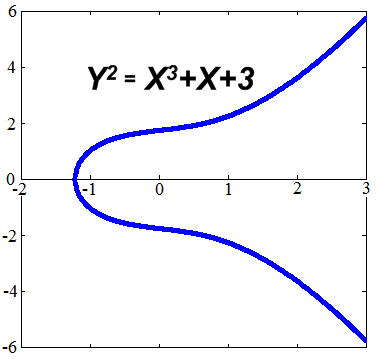
\includegraphics[height=.75\textheight]{pict/elliptic} }
            \mode<article>{ 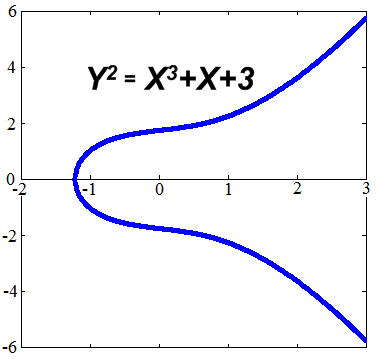
\includegraphics[width=.7\textwidth]{pict/elliptic} } 
            \caption{Кривая $Y^2=X^3+X+3$ в поле действительных чисел}\label{pict:elliptic}
        \end{center}
    \end{figure} 
    \mode<article>{см. рис. \ref{pict:elliptic}}
\end{frame}


\begin{frame}
    \frametitle{Пример кривой $Y^2\equiv X^3+X+3\pmod{7}$}

    \begin{figure}
        \begin{center}
            \mode<presentation>{ 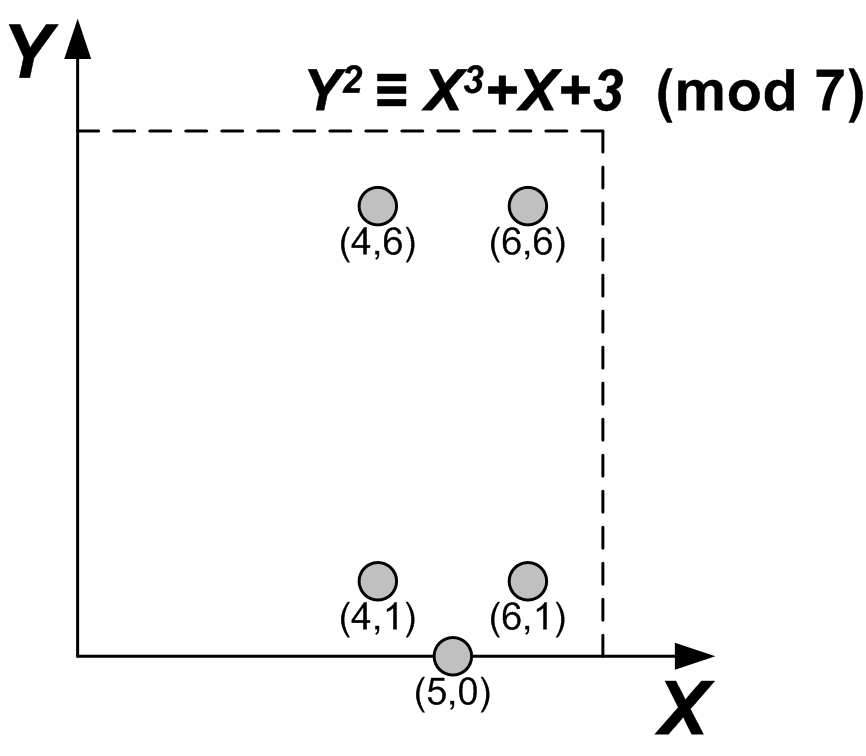
\includegraphics[height=.75\textheight]{pict/y2x3x13mod7} }
            \mode<article>{ 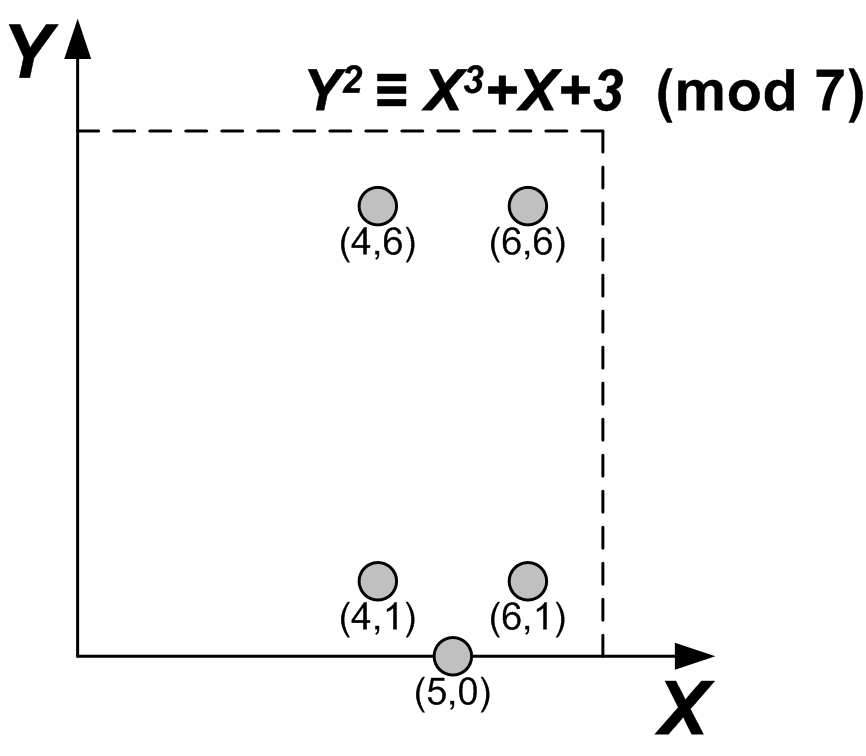
\includegraphics[width=.7\textwidth]{pict/y2x3x13mod7} } 
            \caption{Кривая $Y^2\equiv X^3+X+3\pmod{7}$}\label{pict:y2x3x13mod7}
        \end{center}
    \end{figure} 
    \mode<article>{см. рис. \ref{pict:y2x3x13mod7}}
\end{frame}


\begin{frame}
    \frametitle{Пример кривой $Y^2\equiv X^3+6X+4\pmod{7}$}

    \begin{figure}
        \begin{center}
            \mode<presentation>{ 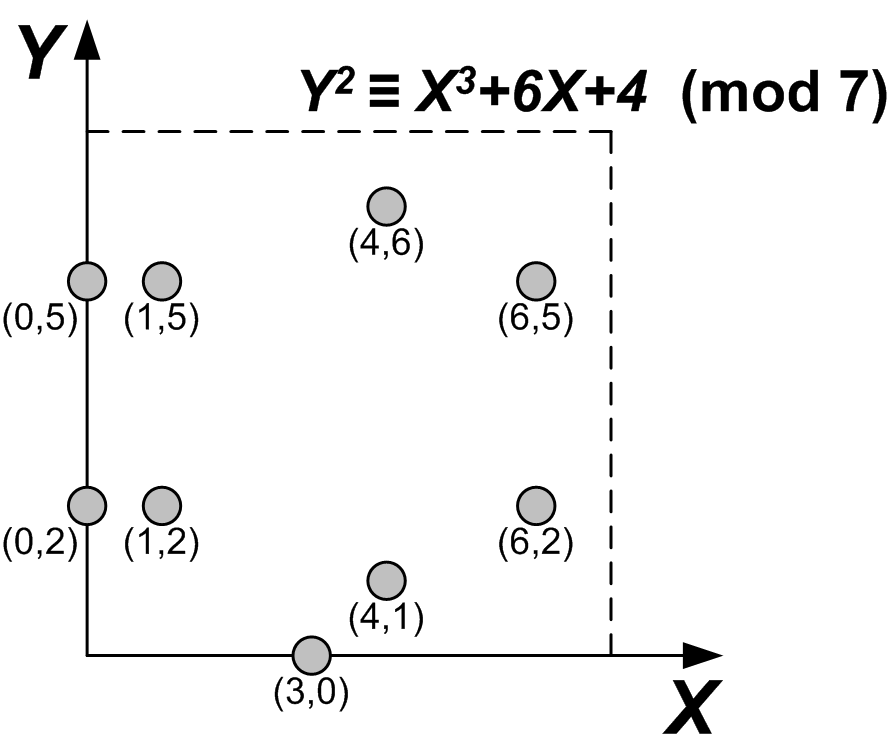
\includegraphics[height=.75\textheight]{pict/y2x36x14mod7} }
            \mode<article>{ 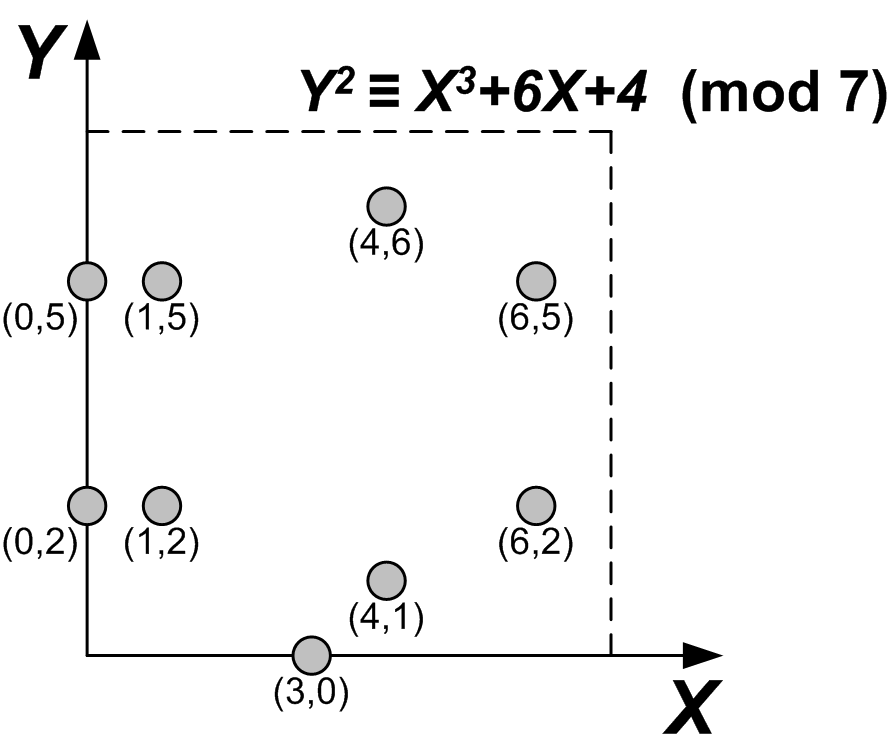
\includegraphics[width=.7\textwidth]{pict/y2x36x14mod7} } 
            \caption{Кривая $Y^2\equiv X^3+6X+4\pmod{7}$}\label{pict:y2x36x14mod7}
        \end{center}
    \end{figure} 
    \mode<article>{см. рис. \ref{pict:y2x36x14mod7}}
\end{frame}


\begin{frame}
    \frametitle{Пример кривой $Y^2\equiv X^3+X\pmod{23}$}

    \begin{figure}
        \begin{center}
            \mode<presentation>{ 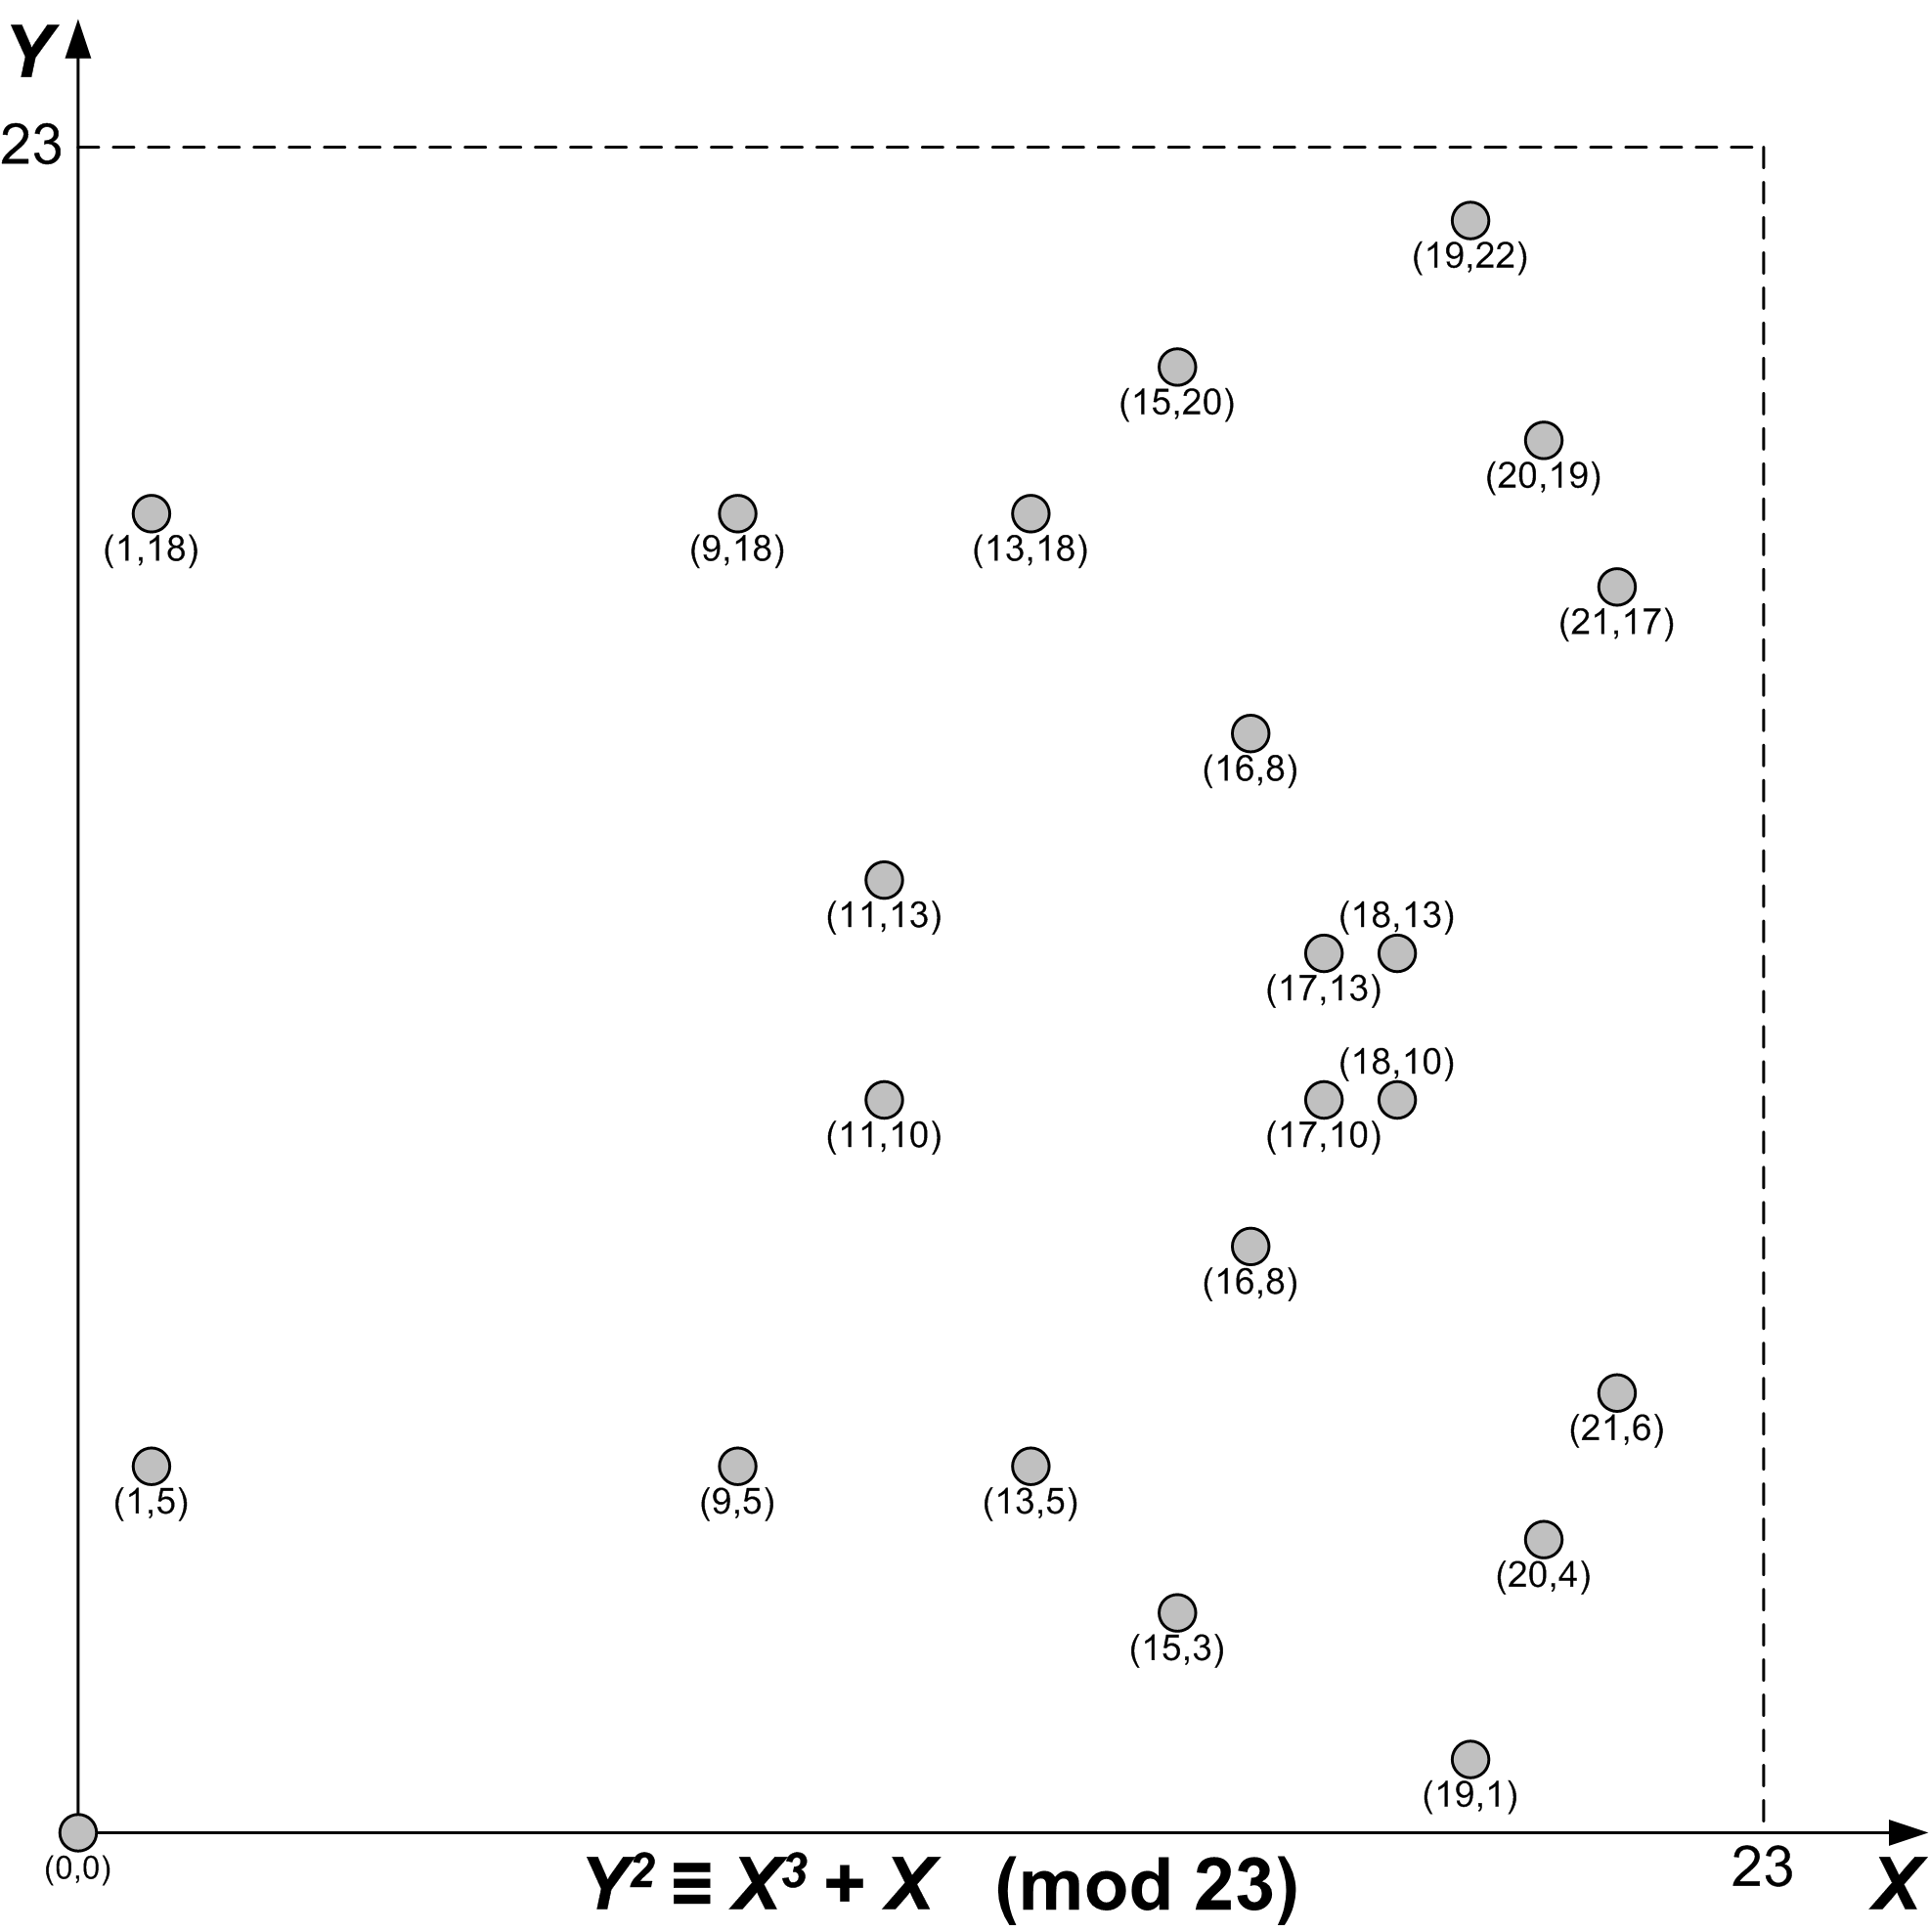
\includegraphics[height=.75\textheight]{pict/y2x31x1mod23} }
            \mode<article>{ 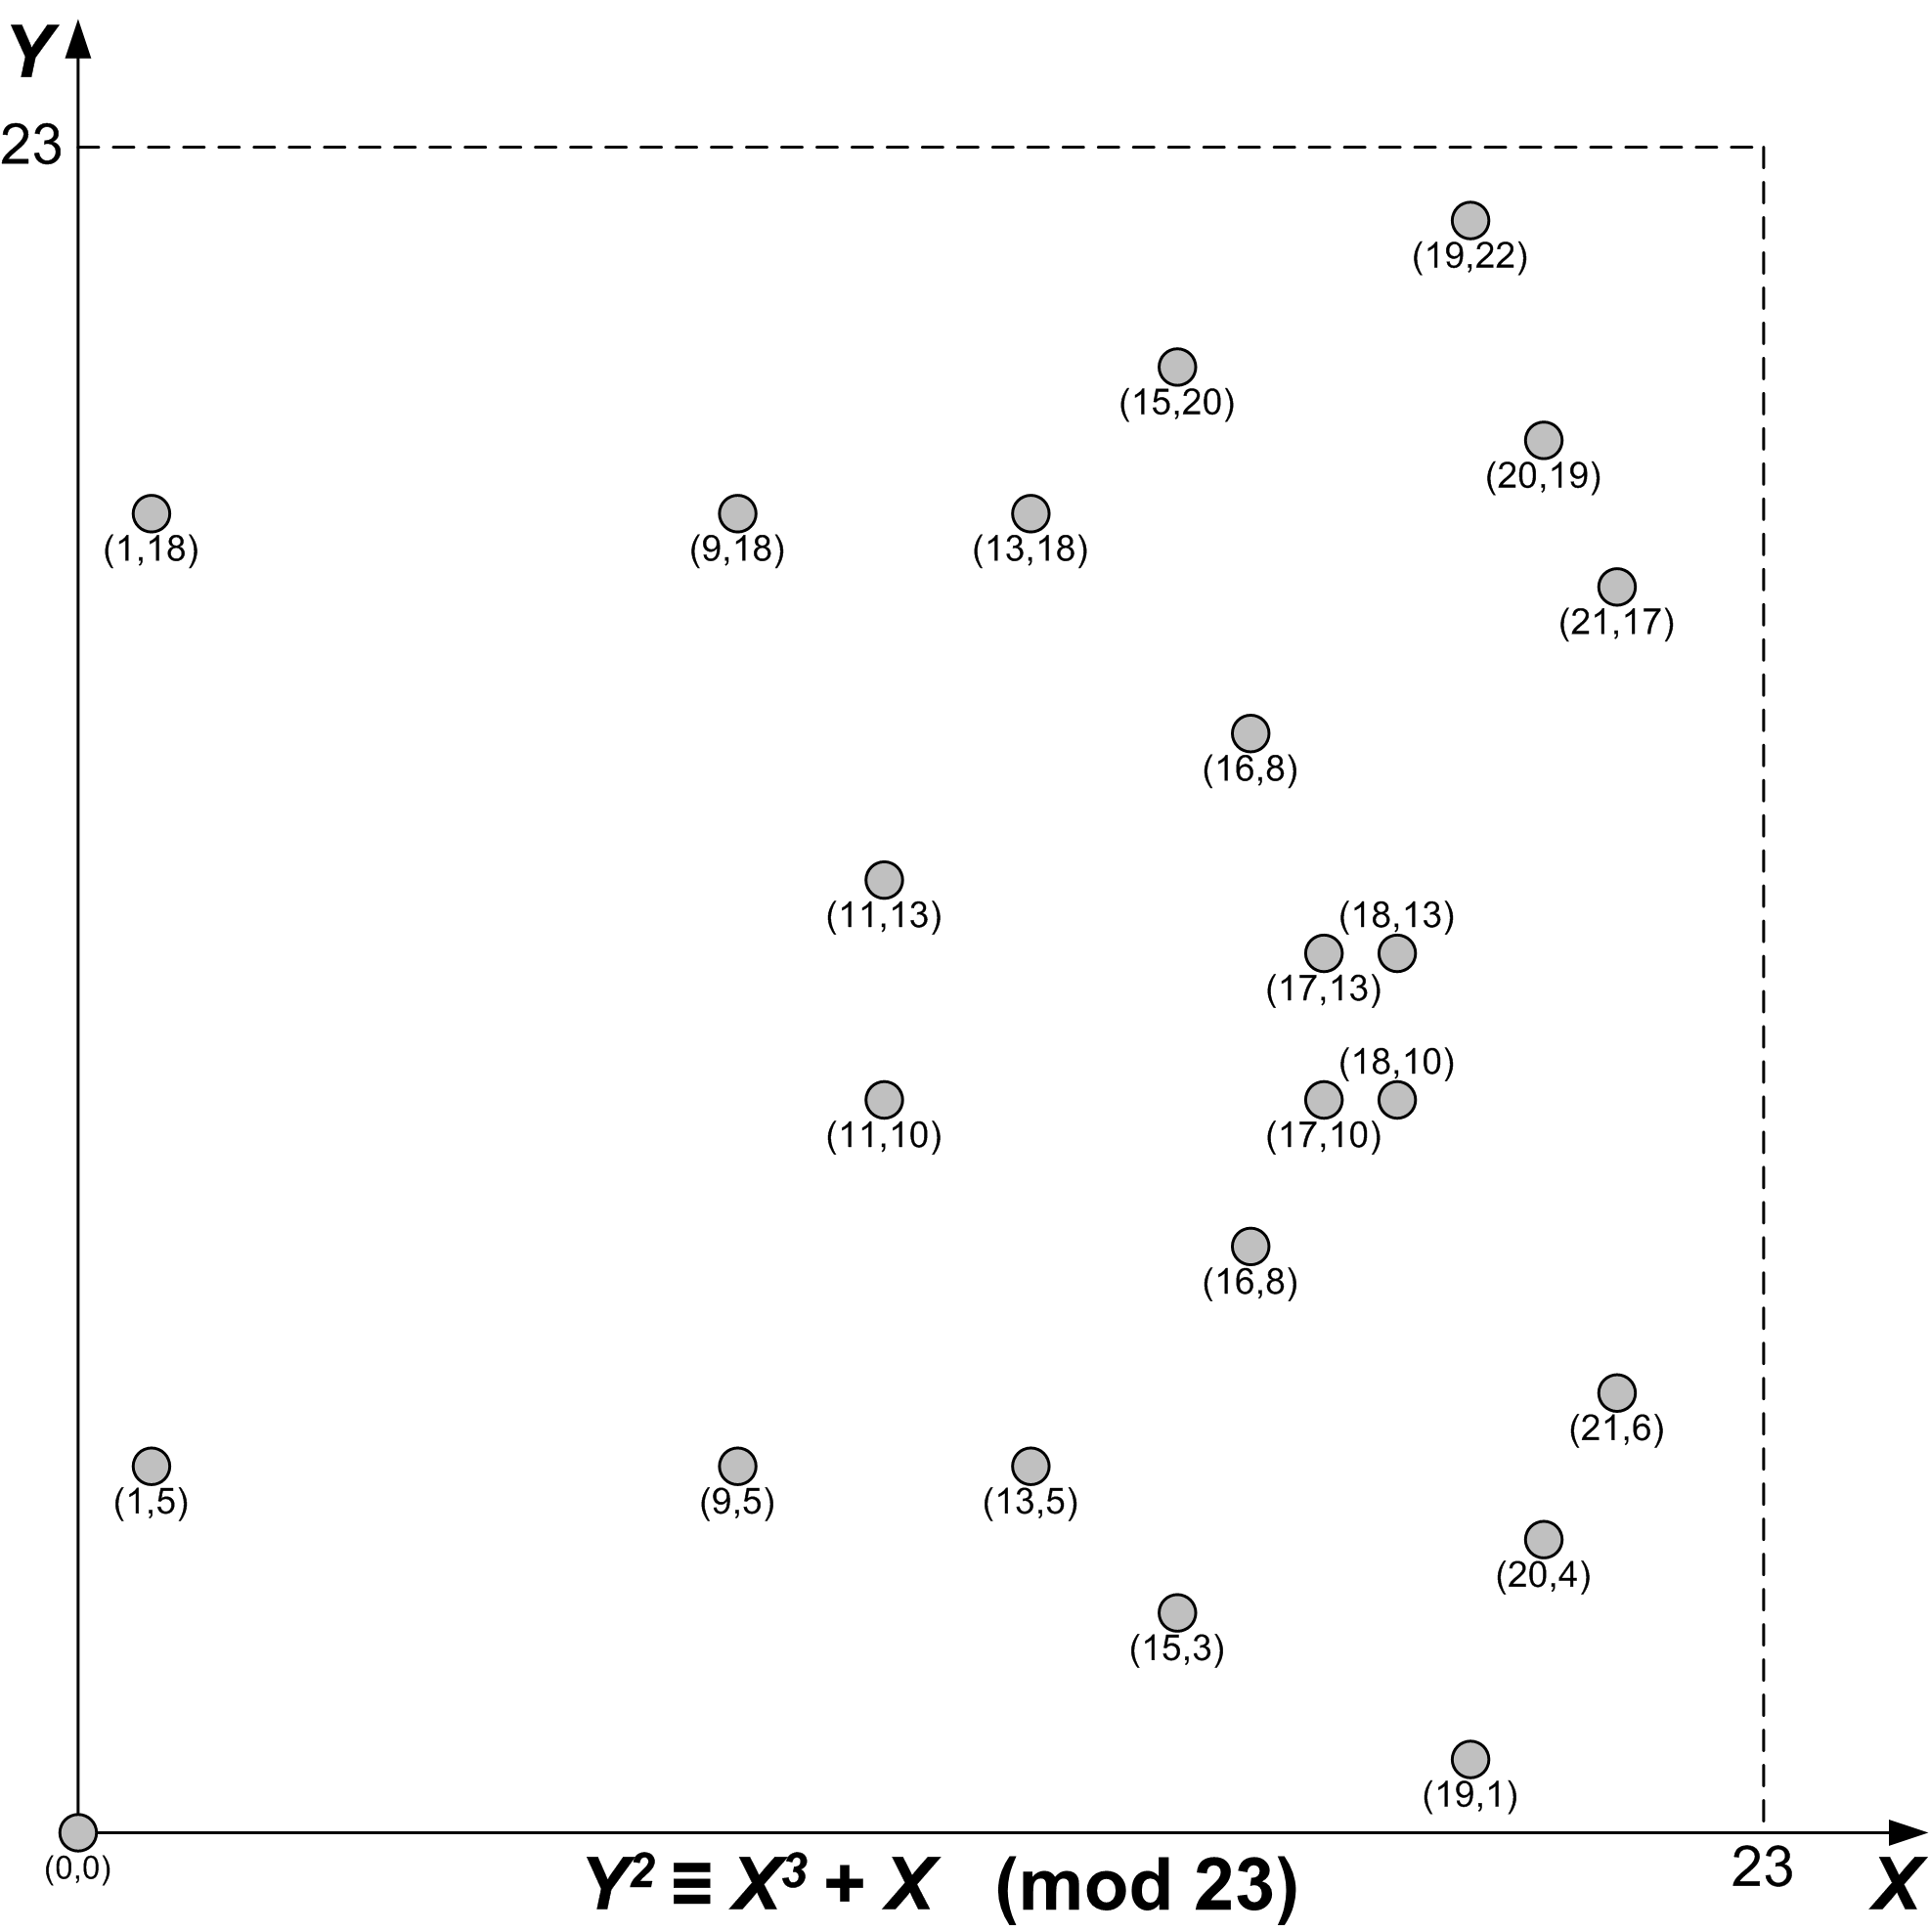
\includegraphics[width=.7\textwidth]{pict/y2x31x1mod23} } 
            \caption{Кривая $Y^2\equiv X^3+X\pmod{23}$}\label{pict:y2x31x1mod23}
        \end{center}
    \end{figure} 
    \mode<article>{см. рис. \ref{pict:y2x31x1mod23}}
\end{frame}


\begin{frame}
    \frametitle{Конечная группа на точках эллиптической кривой}
    \framesubtitle{Множество. Поле $\mathbb{F}_p$}

    \alert{Кривую} \eqref{eq:ellCurveChar3} в поле $\mathbb{F}_p$ можно определить так:
    \begin{equation}\label{eq:ellipticFp}
        E:Y^2\equiv X^3+aX+b \pmod{p},
    \end{equation}
    где константы $a,b$ удовлетворяют\footnote{Дискриминант кубического уравнения} $4a^2+27b^2\not\equiv 0\pmod{p}$. Также вводится понятие \alert{бесконечно удаленной точки} $\mathcal{O}=(x,\infty)$. \alert{Множество}, на котором определяется группа, можно представить так:
    \[
        E=\{P=(x,y)|x,y\in \mathbb{F}_p \text{--- решения \eqref{eq:ellipticFp}}\}\cup\{\mathcal{O}\}
    \]
\end{frame}


\begin{frame}
    \frametitle{Конечная группа на точках эллиптической кривой}
    \framesubtitle{Операция группы. Поле $\mathbb{F}_p$}

    \begin{definition}[Операция $+$ группы, определенной на множестве точек эллиптической кривой <<метод касательных и хорд>>]
        Пусть $P,Q\in E$, $\ell$ --- прямая, соединяющая точки $P$ и $Q$ (если $P=Q$, эта прямая является касательной к \alert{кривой} $E$) и $R$ --- точка пересечения прямой $\ell$ и кривой $E$. Пусть $\ell'$ --- прямая, соединияющая точки $R$ и $\mathcal{O}$. Тогда точка $P+Q$ является такой точкой, что прямая $\ell'$ пересекает \alert{множество} $E$ в точках $R, \mathcal{O}$ и $P+Q$.
    \end{definition}
\end{frame}


Для наглядности в качестве иллюстраций приводятся кривые в поле $\mathbb{R}$, а не $\mathbb{F}_p$.

\begin{frame}
    \frametitle{Иллюстрации к операции $+$ группы. $P+Q$}
    \framesubtitle{Для наглядности приводятся кривые в поле $\mathbb{R}$, а не $\mathbb{F}_p$}

    \begin{figure}
        \begin{center}
            \mode<presentation>{ 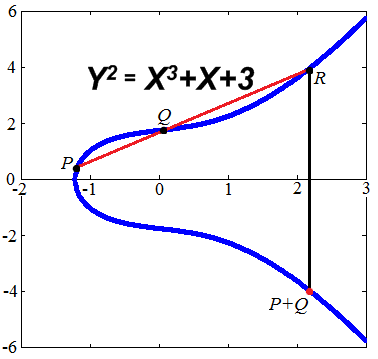
\includegraphics[height=.7\textheight]{pict/ellipticAdd} }
            \mode<article>{ 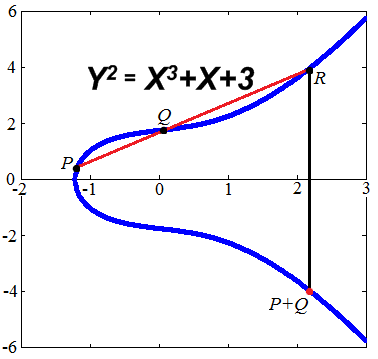
\includegraphics[width=.7\textwidth]{pict/ellipticAdd} } 
            \caption{$P+Q$. Хорда}\label{pict:ellipticAdd}
        \end{center}
    \end{figure} 
    \mode<article>{см. рис. \ref{pict:ellipticAdd}}
\end{frame}


\begin{frame}
    \frametitle{Иллюстрации к операции $+$ группы. $[2]P=P+P$}
    \framesubtitle{Для наглядности приводятся кривые в поле $\mathbb{R}$, а не $\mathbb{F}_p$}

    \begin{figure}
        \begin{center}
            \mode<presentation>{ 
                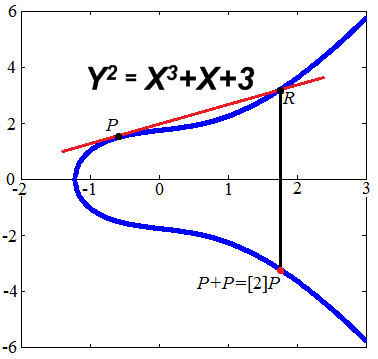
\includegraphics[height=.7\textheight]{pict/elliptic2x} 
            }
            \mode<article>{ 
                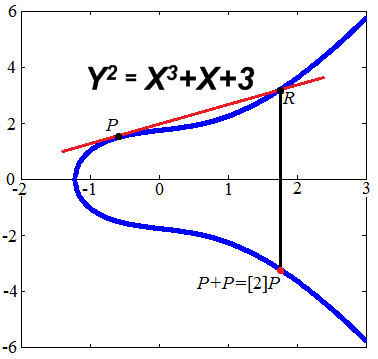
\includegraphics[width=.7\textwidth]{pict/elliptic2x} 
            } 
            \caption{$[2]P=P+P$. Касательная}\label{pict:elliptic2x}
        \end{center}
    \end{figure} 
    \mode<article>{см. рис. \ref{pict:elliptic2x}}
\end{frame}


\begin{frame}
    \frametitle{Операция $+$ группы. $P_3=P_1+P_2$}

    $P+\mathcal{O}=\mathcal{O}+P=P$, $P+(-P)=\mathcal{O}$, где $-P=(x,-y)$ при $P=(x,y)$.
    
    Пусть $P_1=(x_1, y_1)$, $P_2=(x_2, y_2)$, $P_3=(x_3, y_3)$. Хорда (касательная) будет задаваться формулой:
    \[\ell:y-y_1=\lambda(x-x_1),\]
    где 
    \[
        \lambda = 
        \begin{cases}
            \displaystyle
            \frac{y_1-y_2}{x_1-x_2},\text{если $x_1\neq x_2$ (хорда)},\\
            \displaystyle
            \frac{3x_1^2+a}{2y_1},\text{если $x_1=x_2$ или $y_1=y_2\neq 0$ (касательная)}.
        \end{cases}
    \]
\end{frame}


\begin{frame}
    \frametitle{Операция $+$ группы. $P_3=P_1+P_2$}
    Так как пересечение 
    \[
        \ell\cap E:(\lambda(x-x_1)+y_1)^2-(x^3+ax+b)=0
    \]
    есть кубический полином, имеющий три корня: $x_1,x_2,x_3$, что позволяет его записать как
    \[
        c(x-x_1)(x-x_2)(x-x_3)=0,
    \] где $c=-1$. То отсюда получаем $P_3=(x_3,y_3)$:
    \[x_3=\lambda^2-x_1-x_2,\]
    \[y_3=\lambda(x_1-x_3)-y_1.\]
\end{frame}


\begin{frame}
    \frametitle{Эллиптическая кривая $Y^2\equiv X^3+X+3\pmod{7}$}
    \framesubtitle{Пример сложения точек}
    
    Кривой принадлежат, например, точки $(4,1), (6,1), (5,0)$.
    \begin{example}
        Найти $(4,1)+(6,1)$. $\lambda=\frac{3\cdot 4^2+1}{2\cdot 1}=\frac{3\cdot 2 + 1}{2}=\frac{0}{2}=0$. $x_3=0-4-6=3+1=4$, $y_3=0-1=6$. $(4,1)+(6,1)=(4,6)$.
    \end{example}
    
    \begin{example}
        Найти $(4,1)+(5,0)$. $\lambda=\frac{1-0}{4-5}=\frac{1}{6}=1\cdot 6^{-1}=1\cdot 6=6$. $x_3=6^2-4-5=36-9=27=6$, $y_3=6\cdot(4-6)-1=6\cdot 5-1=29=1$. $(4,1)+(5,0)=(6,1)$.
    \end{example}
\end{frame}


\begin{frame}
    \frametitle{Эллиптическая кривая $Y^2\equiv X^3+X+3\pmod{7}$}
    \framesubtitle{Пример сложения точек}
    
    Сведем результаты в таблицу сложения.
    \begin{table}[ht]
        \caption{Сложение точек кривой $Y^2\equiv X^3+X+3\pmod{7}$}\label{t:ellipticAddEx}
        \centering
        \begin{tabular}[c]{|c||c|c|c|c|c|c|}
            \hline
            +               &$\mathcal{O}$  &$(4,1)$        &$(6,6)$        &$(5,0)$        &$(6,1)$        &$(4,6)$\\ \hline\hline 
            $\mathcal{O}$   &$\mathcal{O}$  &$(4,1)$        &$(6,6)$        &$(5,0)$        &$(6,1)$        &$(4,6)$\\ \hline
            $(4,1)$         &$(4,1)$        &$(6,6)$        &$(5,0)$        &$(6,1)$        &$(4,6)$        &$\mathcal{O}$\\ \hline
            $(6,6)$         &$(6,6)$        &$(5,0)$        &$(6,1)$        &$(4,6)$        &$\mathcal{O}$  &$(4,1)$\\ \hline
            $(5,0)$         &$(5,0)$        &$(6,1)$        &$(4,6)$        &$\mathcal{O}$  &$(4,1)$        &$(6,6)$\\ \hline
            $(6,1)$         &$(6,1)$        &$(4,6)$        &$\mathcal{O}$  &$(4,1)$        &$(6,6)$        &$(5,0)$\\ \hline
            $(4,6)$         &$(4,6)$        &$\mathcal{O}$  &$(4,1)$        &$(6,6)$        &$(5,0)$        &$(6,1)$\\ \hline
        \end{tabular}
    \end{table}
    \mode<article>{(см. табл. \ref{t:ellipticAddEx})}
    Видно, что в полученной абелевой группе \alert{образующим} элементом является точка \uncover<2->{$(4,1)$.}
\end{frame}


\begin{frame}
    \frametitle{Умножение точек эллиптической кривой}

    Пусть $m$ --- целое число, а $P\in E$. Вводится
    \[
        [m]P = 
        \begin{cases}
            \displaystyle
            \underbrace{P+P+\cdots+P}_m, \text{для $m>0$},\\
            \mathcal{O}, \text{для $m=0$},\\
            [-m](-P), \text{для $m<0$},
        \end{cases}
    \] где $P=(x,y)$ --- точка кривой, а $-P=(x,-y)$ --- обратный элемент к $P$, так как $P+(-P)=\mathcal{O}$.
\end{frame}


\begin{frame}
    \frametitle{Умножение точек эллиптической кривой}

    Пусть $m$ --- целое \alert{положительное} число, а $P\in E$. Функция $ECMul(P,m)$, возвращающая $[m]P$ может быть определена рекурсивно так:
    \[
        ECMul(P, m) = 
        \begin{cases}
            \mathcal{O}, \text{при $m=0$},\\
            ECMul(P+P, \lfloor m/2 \rfloor),\text{при $m\equiv 0\pmod{2}$},\\
            P+ECMul(P+P, \lfloor m/2 \rfloor),\text{иначе}.
        \end{cases}
    \]
    
    Видно, что умножение точки имеет вычислительную сложность 
    \[
        ECMul(P,m)\in O(\log_2m)
    \]
\end{frame}


\begin{frame}
    \frametitle{Эллиптическая кривая}
    \framesubtitle{Сложные задачи}
    
    Задача \alert{дискретного логарифмирования на эллиптической кривой} (ECDLP\footnote{ECDLP --- elliptic-curve discrete logarithm problem}), заключающаяся в поиске такого $m$ по известным $P$ и $Q$, что справедливо равенство
    
    \[Q=[m]P.\]
    
    ECDLP является трудноразрешимой, если $P$ --- образующий элемент или элемент, порядок которого есть большое простое число.
    
    Координаты $x,y$ точки $P=(x,y)$ есть элементы некоторого поля. На практике активно используются поля арифметики остатков и арифметики полиномов.
\end{frame}


\appendix


\section{$\mathbb{Z}/N\mathbb{Z}$}


\subsection{Расширенный алгоритм Евклида}

\begin{frame}
    \frametitle{Арифметика остатков}
    \framesubtitle{Классический алгоритм Евклида}
    
    \[
    gcd(a, b)=
    \begin{cases}
    b\ \text{при $a=0$},\\
    gcd(b \bmod a, a)\ \text{при $a>0$}.\\
    \end{cases}
    \]

    \begin{example}
        Найти $gcd(210, 119)$.
        \[
        \begin{array}[c]{llll}
         &gcd(210,119)&=gcd(119 \bmod 210, 210)&=\\
        =&gcd(119,210)&=gcd(210\bmod 119, 119)&=\\
        =&gcd(91,119)&=gcd(119 \bmod 91, 91)&=\\
        =&gcd(28,91)&=gcd(91 \bmod 28, 28)&=\\
        =&gcd(7,28)&=gcd(28\bmod 7, 7)&=\\
        =&gcd(0,7) = 7
        \end{array}
        \]
    \end{example}
\end{frame}


\begin{frame}
    \frametitle{Арифметика остатков}
    \framesubtitle{Расширенный алгоритм Евклида}
    
    Расширенный алгоритм Евклида позволяет вычислить 
    \begin{equation}\label{eq:gcdCommon}
        k\cdot a + m\cdot b = gcd(a, b).
    \end{equation}

    Такие алгоритмы называются \alert{самоподтверждающими}. Допустим, что после вычислений компьютер сообщил, что $gcd(a, b)=c$ и что $k\cdot a + m\cdot b=c$. Мы не верим, что $c$ действительно <<наибольший>> общий делитель. Но тогда, если есть общий делитель больше найденного $c$, то он должен делить нацело и $k\cdot a + m\cdot b$ (так как делит и $a$ и $b$). Но так как $k\cdot a + m\cdot b=c$, то <<действительно наибольший>> должен быть \emph{меньше} $c$, чтобы делить его нацело. Конечно для абсолютной уверенности нужно проверить, что $c$ делит $a$ и $b$.

\end{frame}


\begin{frame}
    \frametitle{Арифметика остатков}
    \framesubtitle{Расширенный алгоритм Евклида}
    
    Положим $r_1=a$, $r_0=b$. Тогда 
    \[r_2=b \bmod a=r_0 - \lfloor r_0/r_1\rfloor\cdot r_1,\]
    далее, в полном соответствии с классическим алгоритмом Евклида остатки находятся по формуле:
    \begin{equation}\label{eq:gcdIterative}
        r_{i}=r_{i-2} - \lfloor r_{i-2}/r_{i-1}\rfloor\cdot r_{i-1},
    \end{equation}
    где $i>1$ до тех пор, пока очередной $r_{i}$ не окажется нолём. Тогда $r_{i-1}$ и есть $gcd(a, b)$.
\end{frame}


\begin{frame}
    \frametitle{Арифметика остатков}
    \framesubtitle{Расширенный алгоритм Евклида}
    
    \begin{example}
        Найти $gcd(210, 119)$.
        \[
        \begin{array}[c]{l}
        r_0=119,\\
        r_1=210,\\
        r_2=r_0 - \lfloor r_0/r_1\rfloor\cdot r_1=119-\lfloor 119/210\rfloor\cdot 210=119,\\
        r_3=r_{1} - \lfloor r_{1}/r_{2}\rfloor\cdot r_{2}=210-\lfloor 210/119\rfloor\cdot 119=91,\\
        r_4=r_{2} - \lfloor r_{2}/r_{3}\rfloor\cdot r_{3}=119-\lfloor 119/91\rfloor\cdot 91=28,\\
        r_5=r_{3} - \lfloor r_{3}/r_{4}\rfloor\cdot r_{4}=91-\lfloor 91/28\rfloor\cdot 28=7,\\
        r_6=r_{4} - \lfloor r_{4}/r_{5}\rfloor\cdot r_{5}=28-\lfloor 28/7\rfloor\cdot 7=0,\\
        gcd(210, 119)=r_5=7
        \end{array}
        \]
    \end{example}
\end{frame}


\begin{frame}
    \frametitle{Арифметика остатков}
    \framesubtitle{Расширенный алгоритм Евклида}
    
    Теперь положим, что 
    \begin{equation}\label{eq:gcdDecomp}
        r_i=k_i\cdot a + m_i\cdot b,
    \end{equation}
    где $k_i,m_i$ --- коэффициенты разложения  \eqref{eq:gcdCommon} на $i$-м шаге алгоритма.

    Для $r_0=b$ имеем $k_0=0, m_0=1$. Для $r_1=a$ имеем $k_1=1, m_1=0$.

    Подставляем $r_i$ из формулы \eqref{eq:gcdDecomp} в формулу \eqref{eq:gcdIterative}:
    \[
    k_i\cdot a + m_i\cdot b=(k_{i-2}\cdot a + m_{i-2}\cdot b) - \lfloor r_{i-2}/r_{i-1}\rfloor\cdot (k_{i-1}\cdot a + m_{i-1}\cdot b).
    \]

    Отсюда непосредственно выражаются $k_i$ и $m_i$:
    \[
    \begin{array}[c]{l}
    k_i=k_{i-2}-\lfloor r_{i-2}/r_{i-1}\rfloor\cdot k_{i-1},\\
    m_i=m_{i-2}-\lfloor r_{i-2}/r_{i-1}\rfloor\cdot m_{i-1}.
    \end{array}
    \]
\end{frame}


\begin{frame}
    \frametitle{Арифметика остатков}
    \framesubtitle{Расширенный алгоритм Евклида. Пример}
    
    Найти $gcd(210, 119)=k\cdot 210 + m\cdot 119$. Шаги 0--3.
    \[
        \begin{array}[c]{llll}
        \hline
        r_0&&&=119,\\
        k_0&&&=0,\\
        m_0&&&=1,\\
        \hline
        r_1&&&=210,\\
        k_1&&&=1,\\
        m_1&&&=0,\\
        \hline
        r_2&=r_0 - \lfloor r_0/r_1\rfloor\cdot r_1&=119-\lfloor 119/210\rfloor\cdot 210&=119,\\
        k_2&=k_{0}-\lfloor r_{0}/r_{1}\rfloor\cdot k_{1}&=0-\lfloor 119/210\rfloor\cdot 1&=0,\\
        m_2&=m_{0}-\lfloor r_{0}/r_{1}\rfloor\cdot m_{1}&=1-\lfloor 119/210\rfloor\cdot 0&=1,\\
        \hline
        r_3&=r_{1} - \lfloor r_{1}/r_{2}\rfloor\cdot r_{2}&=210-\lfloor 210/119\rfloor\cdot 119&=91,\\
        k_3&=k_{1}-\lfloor r_{1}/r_{2}\rfloor\cdot k_{2}&=1-\lfloor 210/119\rfloor\cdot 0&=1,\\
        m_3&=m_{1}-\lfloor r_{1}/r_{2}\rfloor\cdot m_{2}&=0-\lfloor 210/119\rfloor\cdot 1&=-1,\\
        \hline
        \end{array}
    \]
\end{frame}


\begin{frame}
    \frametitle{Арифметика остатков}
    \framesubtitle{Расширенный алгоритм Евклида. Пример}
    
    Найти $gcd(210, 119)=k\cdot 210 + m\cdot 119$. Шаги 3--6.
    
    \[
        \begin{array}[c]{llll}
        \hline
        r_4&=r_{2} - \lfloor r_{2}/r_{3}\rfloor\cdot r_{3}&=119-\lfloor 119/91\rfloor\cdot 91&=28,\\
        k_4&=k_{2}-\lfloor r_{2}/r_{3}\rfloor\cdot k_{3}&=0-\lfloor 119/91\rfloor\cdot 1&=-1,\\
        m_4&=m_{2}-\lfloor r_{2}/r_{3}\rfloor\cdot m_{3}&=1-\lfloor 119/91\rfloor\cdot -1&=2,\\
        \hline
        r_5&=r_{3} - \lfloor r_{3}/r_{4}\rfloor\cdot r_{4}&=91-\lfloor 91/28\rfloor\cdot 28&=7,\\
        k_5&=k_{3}-\lfloor r_{3}/r_{4}\rfloor\cdot k_{4}&=1-\lfloor 91/28\rfloor\cdot -1&=4,\\
        m_5&=m_{3}-\lfloor r_{3}/r_{4}\rfloor\cdot m_{4}&=-1-\lfloor 91/28\rfloor\cdot 2&=-7,\\
        \hline
        r_6&=r_{4} - \lfloor r_{4}/r_{5}\rfloor\cdot r_{5}&=28-\lfloor 28/7\rfloor\cdot 7&=0,\\
        k_6&=k_{4}-\lfloor r_{4}/r_{5}\rfloor\cdot k_{5}&=-1-\lfloor 28/7\rfloor\cdot 4&=-17,\\
        m_6&=m_{4}-\lfloor r_{4}/r_{5}\rfloor\cdot m_{5}&=2-\lfloor 28/7\rfloor\cdot -7&=30.\\
        \hline
        \end{array}
    \]
    Получаем результат: $gcd(210, 119)=r_5=k_5\cdot 210 + m_5\cdot 119=4\cdot 210 - 7\cdot 119 = 7.$
\end{frame}


\subsection{Решение уравнения $a\cdot x \equiv b\pmod{N}$}

\begin{frame}
    \frametitle{Решение уравнения $a\cdot x \equiv b\pmod{N}$}
    \framesubtitle{Поиск мультипликативного обратного}
    
    Особенностью уравнения 
    \begin{equation} \label{eq:linearCommon}
        a\cdot x \equiv b\pmod{N}
    \end{equation}
    является то, что оно может иметь ни одного, одно или много решений.

    Рассмотрим решение частного случая --- поиск \alert{мультипликативного обратного}:
    \begin{equation}\label{eq:multiplicativeReversy}
        a\cdot a^{-1} \equiv a^{-1}\cdot a\equiv 1\pmod{N}
    \end{equation}
    при этом $gcd(a, N)=1$. Расширенный алгоритм Евклида дает
    \[gcd(a, N)\equiv k\cdot a + m\cdot N\equiv k\cdot a \equiv a\cdot k \equiv 1 \pmod{N}\]
    и таким образом $k$ и есть искомый \alert{мультипликативный обратный} $a^{-1}$.
\end{frame}

Кстати, если взять простое $N$ (которое конечно является взаимно простым с числами $y\in[0,N-1]$), то в таком кольце вычетов $\mathbb{Z}/N\mathbb{Z}$ мультипликативный обратный есть всегда. Тогда можно определить операцию деления на $a$, как операцию умножения на мультипликативный обратный элемент $a^{-1}$.



\begin{frame}
    \frametitle{Решение уравнения $a\cdot x \equiv b\pmod{N}$}
    \framesubtitle{Решение в общем виде}
    
    \begin{enumerate}
    \item \label{en:linearModNoneDecision}
    Если $gcd(a,N)=1$, то существует ровно одно решение. Оно может быть найдено с помощью мультипликативного обратного $c$, удовлетворяющего $a\cdot c\equiv 1\pmod{N}$. В этом случае $x\equiv c\cdot b\pmod{N}$.

    \item Если $gcd(a,N)\neq 1$ и $g=gcd(a,N)$ делит $b$ нацело, то существует $g$ решений. Чтобы их найти нужно разделить исходное уравнение на $g$:
    \[a'\cdot x' \equiv b' \pmod{N'},\] где $a'=\frac{a}{g}$, $b'=\frac{b}{g}$, $N'=\frac{N}{g}$. Случай сведен к случаю $gcd(a',N')=1$ и $x'$ находится в соответствии с пунктом \ref{en:linearModNoneDecision}.
    \[x=x'+i\cdot N',\] где $i\in [0,g-1]$.
    
    \item В других случаях решений нет.
    \end{enumerate}
\end{frame}


\begin{frame}
    \frametitle{Пример. Уравнение $21\cdot x \equiv 15 \pmod{39}$.}

    Применяя алгоритм Евклида, находим:
    \[
        \begin{array}[c]{rlll}
        g=&gcd(21,39)&=gcd(39 \bmod 21, 21)&=\\
        =&gcd(18,21)&=gcd(21\bmod 18, 18)&=\\
        =&gcd(3,18)&=gcd(18 \bmod 3, 3)&=\\
        =&gcd(0,3)&=3
        \end{array}
    \]
    
    $g=3$ делит $b=15$ без остатка. Делим исходное выражение на $g$:
    \[
        \begin{array}[c]{c}
            \displaystyle
            \frac{21}{3}\cdot x' \equiv \frac{15}{3} \pmod{\frac{39}{3}},\\
            \\
            7\cdot x' \equiv 5 \pmod{13}.
        \end{array}
    \]    
    Для поиска решения $c$ уравнения \ref{eq:multiplicativeReversy} т.е. $7\cdot c\equiv 1 \pmod{13}$ применим расширенный алгоритм Евклида для поиска $gcd(7,13)$.
\end{frame}


\begin{frame}
    \frametitle{Пример. Уравнение $21\cdot x \equiv 15 \pmod{39}$.}
    
    \[
        \begin{array}[c]{llll}
            \hline
            r_0&&&=13,\\
            k_0&&&=0,\\
            m_0&&&=1,\\
            \hline
            r_1&&&=7,\\
            k_1&&&=1,\\
            m_1&&&=0,\\
            \hline
            r_2&=r_0 - \lfloor r_0/r_1\rfloor\cdot r_1&=13-\lfloor 13/7\rfloor\cdot 7&=6,\\
            k_2&=k_{0}-\lfloor r_{0}/r_{1}\rfloor\cdot k_{1}&=0-\lfloor 13/7\rfloor\cdot 1&=-1,\\
            m_2&=m_{0}-\lfloor r_{0}/r_{1}\rfloor\cdot m_{1}&=1-\lfloor 13/7\rfloor\cdot 0&=1,\\
            \hline
        \end{array}
    \]
\end{frame}


\begin{frame}
    \frametitle{Пример. Уравнение $21\cdot x \equiv 15 \pmod{39}$.}
    
    \[
        \begin{array}[c]{llll}
            \hline
            r_3&=r_{1} - \lfloor r_{1}/r_{2}\rfloor\cdot r_{2}&=7-\lfloor 7/6\rfloor\cdot 6&=1,\\
            k_3&=k_{1}-\lfloor r_{1}/r_{2}\rfloor\cdot k_{2}&=1-\lfloor 7/6\rfloor\cdot -1&=2,\\
            m_3&=m_{1}-\lfloor r_{1}/r_{2}\rfloor\cdot m_{2}&=0-\lfloor 7/6\rfloor\cdot 1&=-1,\\
            \hline
            r_4&=r_{2} - \lfloor r_{2}/r_{3}\rfloor\cdot r_{3}&=6-\lfloor 6/1\rfloor\cdot 1&=0,\\
            k_4&=k_{2}-\lfloor r_{2}/r_{3}\rfloor\cdot k_{3}&=-1-\lfloor 6/1\rfloor\cdot 2&=-13,\\
            m_4&=m_{2}-\lfloor r_{2}/r_{3}\rfloor\cdot m_{3}&=1-\lfloor 6/1\rfloor\cdot -1&=7,\\
            \hline
        \end{array}
    \]
    $c=k_3=2$. Проверим: $7\cdot 2 \equiv 1 \pmod{13}$. 

    Далее $x'\equiv c\cdot b'\equiv2\cdot 5\equiv 10\pmod{13}$. Проверим: $7\cdot 10\equiv 5\pmod{13}$.

    Исходное уравнение имеет $g=3$ решения: $x=10+i\cdot 13$, $0\leq i<3$. 
    \[x\in\{10, 23, 36\}.\]
    
\end{frame}


\subsection{Быстрое возведение в степень}


\begin{frame}
    \frametitle{Быстрое возведение в степень}
    
    Задача дискретного логарифмирования, заключающаяся в поиске показателя степени $x$, при известных $y$, $a$, $N$ выражения 
    \[y\equiv a^x \pmod{N}.\]
    Рассмотрим способ быстрого возведения в степень, то есть поиска $y$ по известным $x$, $a$, $N$. Можно выполнить:
    \[y\equiv\underbrace{a\cdot a\cdot\ldots\cdot a\cdot a}_{x}\pmod{N},\]
    но это займет слишком много времени при больших $x$.
\end{frame}

\begin{frame}
    \frametitle{Быстрое возведение в степень}
    
    Представим $x$ в двоичной системе счисления:
    \[x=\sum_{i=0}^{m}b_i\cdot 2^i.\]

    Тогда:\[y \equiv a^{\sum_{i=0}^{m} b_i\cdot 2^i} \equiv \prod_{i=0}^{m}a^{b_i\cdot 2^i}\pmod{N}.\]
    
    Введем обозначение $t_i=a^{2^i}$. При этом: 
    \[y\equiv\prod_{i=0}^{m}(1+b_i\cdot(t_i-1))\pmod{N}.\]

\end{frame}


\begin{frame}
    \frametitle{Быстрое возведение в степень}
    
    Заметим, что: 
    \[t_i=a^{2^i}=a^{2\cdot 2^{i-1}}=a^{ 2^{i-1}}\cdot a^{2^{i-1}}= t_{i-1}\cdot t_{i-1}=t_{i-1}^2.\]

    Итак, рекуррентность:
    \[
        t_i=
        \begin{cases}
        a,\ \text{при $i=0$},\\
        t_{i-1}^2 \pmod{N},\ \text{при $i>0$}.
        \end{cases}
    \]
\end{frame}


\begin{frame}
    \frametitle{Алгоритм быстрого возведения в степень}
    
    \begin{enumerate}
        \item Находится двоичное представление числа $x$: 
        \[x\equiv(b_mb_{m-1}\cdots b_1b_0)_2.\]

        Устанавливается $i=0, t_0=a, y=1$.
        \item \label{en:algQuickPower}
        Находится $z\equiv y\cdot (1+b_i\cdot(t_i-1))\pmod{N}$. Далее $y=z, i=i+1$.
        \[t_i=t_{i-1}^2\pmod{N}.\]

        \item Если $i>m$ то $y$ найдено, иначе перехдим к пункту \ref{en:algQuickPower}.
    \end{enumerate}
\end{frame}
    

\begin{frame}
    \frametitle{Пример. Найти $y\equiv 89^{177}\pmod{613}$}

    $177 \equiv (10110001)_2$
    \[
        \begin{array}[c]{|c|l|c|l|}
            \hline\hline
            i & t_i & b_i & y\\
            \hline\hline
            0&89&1&89\\
            \hline
            1&89^2\equiv 565\pmod{613}&0&89\cdot 1\equiv 89\pmod{613}\\
            \hline
            2&565^2\equiv 465\pmod{613}&0&89\cdot 1\equiv 89\pmod{613}\\
            \hline
            3&465^2\equiv 449\pmod{613}&0&89\cdot 1\equiv 89\pmod{613}\\
            \hline
            4&449^2\equiv 537\pmod{613}&1&89\cdot 537\equiv 592\pmod{613}\\
            \hline
            5&537^2\equiv 259\pmod{613}&1&592\cdot 259\equiv78\pmod{613}\\
            \hline
            6&259^2\equiv 264\pmod{613}&0&78\cdot 1\equiv 78\pmod{613}\\
            \hline
            7&264^2\equiv 427\pmod{613}&1&78\cdot 427\equiv 204\pmod{613}\\
            \hline
        \end{array}
    \]

    Ответ: $y=204$. Вместо $177$ последовательных умножений по модулю обошлись шестнадцатью. В общем случае выигрыш по количеству умножений можно оценить как $2\cdot \lceil\log_2(x)\rceil$
\end{frame}

\begin{frame}
    \frametitle{Источники}
    
    Представление об арифметике полиномов и модулярной арифметике можно получить из \cite{bib:knuth:artOfProgramming2}.
    Краткий обзор математических основ криптографии в \cite{bib:smart:crypto, bib:mao:modernCrypto}.
    Для подробного изучения теории по применению эллиптических кривых в криптографии можно рекомендовать \cite{bib:bolotov:elliptic}.
\end{frame}


\begin{frame}[allowframebreaks]{Библиография}
    \bibliographystyle{gost780u}
    \bibliography{./../bibliobase}
\end{frame}

\end{document}